% lecture17.tex — Vector Fields and the Poincaré–Hopf Theorem

\section{Vector Fields and the Poincar\'e--Hopf Theorem}

\begin{definition}{Vector Field}{vector-field}
    A \emph{vector field} on a manifold $M$ is a smooth section $v \colon M \to TM$, i.e.\ a smooth assignment of a tangent vector $v(x) \in T_x M$ at each point $x \in M$.
\end{definition}

If $v(x) \neq 0$ at some point $x \in M$, then $v$ is nearly constant in magnitude and direction near $x$.

\begin{center}
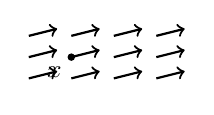
\begin{tikzpicture}[scale=0.9]
    \foreach \y in {-0.3, 0, 0.3} {
        \foreach \x in {-0.6, 0, 0.6, 1.2} {
            \draw[->,thick] (\x,\y) -- (\x+0.4,\y+0.1);
        }
    }
    \fill (0,0) circle (1.5pt) node[below left] {\small $x$};
\end{tikzpicture}
\end{center}

However, if $v(x) = 0$, $v$ can behave interestingly around such \emph{zeros}.

\begin{example}{Behaviors of Vector Fields Near Zeros}{vf-behaviors}
    On a surface, some possible behaviors of $v$ around its zeros include: sink, source, circulation, spiral, and saddle.
\end{example}

\begin{center}
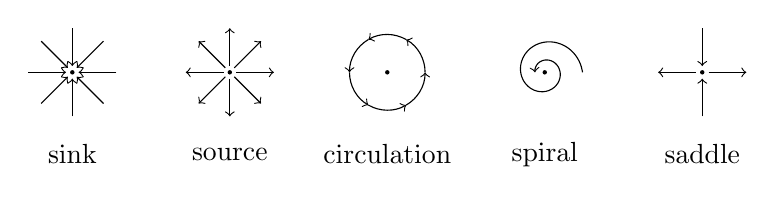
\begin{tikzpicture}[scale=0.8]
    % Sink
    \node at (0,-1.3) {sink};
    \fill (0,0) circle (1pt);
    \foreach \a in {0,45,90,135,180,225,270,315} {
        \draw[->] ({0.7*cos(\a)},{0.7*sin(\a)}) -- ({0.1*cos(\a)},{0.1*sin(\a)});
    }
    % Source
    \begin{scope}[xshift=2.5cm]
        \node at (0,-1.3) {source};
        \fill (0,0) circle (1pt);
        \foreach \a in {0,45,90,135,180,225,270,315} {
            \draw[->] ({0.1*cos(\a)},{0.1*sin(\a)}) -- ({0.7*cos(\a)},{0.7*sin(\a)});
        }
    \end{scope}
    % Circulation
    \begin{scope}[xshift=5cm]
        \node at (0,-1.3) {circulation};
        \fill (0,0) circle (1pt);
        \draw[->] (0.6,0) arc(0:60:0.6);
        \draw[->] (0.3,0.52) arc(60:120:0.6);
        \draw[->] (-0.3,0.52) arc(120:180:0.6);
        \draw[->] (-0.6,0) arc(180:240:0.6);
        \draw[->] (-0.3,-0.52) arc(240:300:0.6);
        \draw[->] (0.3,-0.52) arc(300:360:0.6);
    \end{scope}
    % Spiral
    \begin{scope}[xshift=7.5cm]
        \node at (0,-1.3) {spiral};
        \fill (0,0) circle (1pt);
        \draw[->,domain=0:540,smooth,variable=\t,samples=60]
            plot ({0.6*exp(-\t/400)*cos(\t)},{0.6*exp(-\t/400)*sin(\t)});
    \end{scope}
    % Saddle
    \begin{scope}[xshift=10cm]
        \node at (0,-1.3) {saddle};
        \fill (0,0) circle (1pt);
        \draw[->] (0,0.7) -- (0,0.1);
        \draw[->] (0,-0.7) -- (0,-0.1);
        \draw[->] (0.1,0) -- (0.7,0);
        \draw[->] (-0.1,0) -- (-0.7,0);
    \end{scope}
\end{tikzpicture}
\end{center}

We'll see that the zeros of $v$ encode some information on the topology of the manifold $M$!

\subsection{Index of a Vector Field}

Suppose $v$ is a vector field on $\R^m$ that has an isolated zero at the origin $0 \in \R^m$. Then, for any small enough radius $\varepsilon > 0$, $v$ has no zeros except at the origin inside the sphere $S_\varepsilon^{m-1}$ of radius $\varepsilon$ around the origin.

\begin{definition}{Index of a Vector Field at a Zero}{index-vf}
    The \emph{index} of $v$ at $0$, $\ind_0(v)$, is the degree of the directional map
    \[
        S_\varepsilon^{m-1} \to S^{m-1}, \quad x \mapsto \frac{v(x)}{|v(x)|}.
    \]
\end{definition}

\begin{example}{Index in Two Dimensions}{index-2d}
    In the two-dimensional case, $\ind_x(v)$ simply counts the number of times $v$ rotates (in the counterclockwise direction) as we walk counterclockwise around the circle. For example, a sink, source, circulation, and spiral each have index $+1$; a saddle has index $-1$; and a ``double rotation'' has index $+2$.
\end{example}

More generally, if $x$ is an isolated zero of a vector field $v$ on $M$, then we can define $\ind_x(v)$ to be the index of the pushforward vector field $\varphi_*^{-1}(v)$ at $0$, where $\varphi \colon U \to M$, $0 \mapsto x$, is a local parametrization.

\subsection{Poincar\'e--Hopf Theorem}

\begin{theorem}{Poincar\'e--Hopf Index Theorem}{poincare-hopf}
    If $v$ is a smooth vector field on a compact, oriented manifold $M$ with only finitely many zeros, then
    \[
        \chi(M) = \sum_{v(x) = 0} \ind_x(v).
    \]
\end{theorem}

\begin{corollary}{Hairy Ball Theorem}{hairy-ball}
    There is no nowhere-vanishing vector field on $S^2$, since $\chi(S^2) = 2 \neq 0$.

    ``You can't comb a hairy ball without leaving a bald spot.''
\end{corollary}

\begin{proof}[Proof of Poincar\'e--Hopf]
    The idea is that a vector field determines a flow
    \[
        f_t \colon M \to M
    \]
    that is homotopic to $f_0 = \id$, and tangent to $v$ at time zero. Such a family of maps can be obtained by solving the ODE given by the vector field. Another way is to simply take $f_t(x) = \pi(x + t v(x))$, where $\pi$ is the projection map from the $\varepsilon$-neighborhood theorem.

    For small $t > 0$, fixed points of $f_t$ correspond exactly to zeros of $v$, so it suffices to prove that $\ind_x(v) = L_x(f_t)$.

    This is a local problem, so we may work in $\R^m$. From basic calculus, there is a smooth vector-valued function $r(t, x)$ such that
    \[
        f_t(x) = f_0(x) + t f_0'(x) + t^2 r(t, x) = f_0(x) + t v(x) + t^2 r(t, x),
    \]
    so
    \[
        \frac{f_t(x) - x}{|f_t(x) - x|} = \frac{v(x) + t r(t, x)}{|v(x) + t r(t, x)|} \colon S_\varepsilon^{m-1} \to S^{m-1}
    \]
    is homotopic to $v(x)/|v(x)|$, whose degree is $\ind(v)$.

    On the other hand, the local Lefschetz number $L_x(f_t)$ is the degree of the map
    \[
        \partial B_\varepsilon^m \to S^{m-1}, \quad z \mapsto \frac{f_t(z) - z}{|f_t(z) - z|}.
    \]
    For Lefschetz fixed points, simple linear algebra shows that this agrees with the previous definition, since $\deg\!\left(z \mapsto \frac{(A - I)z}{|(A - I)z|}\right) = \sign \det(A - I)$.

    Homotopy invariance follows from the boundary theorem.
\end{proof}

\begin{corollary}{Euler Characteristic via Self-Intersection}{euler-self-intersection}
    $\chi(M) = I(M, M)$, where $M$ is considered as the $0$-section $M \subset TM$.
\end{corollary}
